%%%%%%%%%%%%%%%%%%%%%%%%%%%%%%%%%%%%%%%%%
% Academic Title Page
% LaTeX Template
% Version 2.0 (17/7/17)
%
% This template was downloaded from:
% http://www.LaTeXTemplates.com
%
% Original author:
% WikiBooks (LaTeX - Title Creation) with modifications by:
% Vel (vel@latextemplates.com)
%
% License:
% CC BY-NC-SA 3.0 (http://creativecommons.org/licenses/by-nc-sa/3.0/)
% 
% Instructions for using this template:
% This title page is capable of being compiled as is. This is not useful for 
% including it in another document. To do this, you have two options: 
%
% 1) Copy/paste everything between \begin{document} and \end{document} 
% starting at \begin{titlepage} and paste this into another LaTeX file where you 
% want your title page.
% OR
% 2) Remove everything outside the \begin{titlepage} and \end{titlepage}, rename
% this file and move it to the same directory as the LaTeX file you wish to add it to. 
% Then add \input{./<new filename>.tex} to your LaTeX file where you want your
% title page.
%
%%%%%%%%%%%%%%%%%%%%%%%%%%%%%%%%%%%%%%%%%

%----------------------------------------------------------------------------------------
%	PACKAGES AND OTHER DOCUMENT CONFIGURATIONS
%----------------------------------------------------------------------------------------

\documentclass[11pt]{article}

\usepackage[utf8]{inputenc} % Required for inputting international characters
\usepackage[T1]{fontenc} % Output font encoding for international characters
\usepackage{graphicx}
\usepackage{mathpazo} % Palatino font
\usepackage[legalpaper,margin=0.9in] {geometry}
\usepackage{fancyhdr}
\usepackage{float}

\setcounter{tocdepth}{4}
\setcounter{secnumdepth}{4}


\pagestyle{fancy}
\fancyhf{}
\lhead{\textsc{University of Regina}}
\rhead{\textsc{Software Systems Engineering}}
\cfoot{\thepage}

\begin{document}

%----------------------------------------------------------------------------------------
%	TITLE PAGE
%----------------------------------------------------------------------------------------

\begin{titlepage} % Suppresses displaying the page number on the title page and the subsequent page counts as page 1
	\newcommand{\HRule}{\rule{\linewidth}{0.5mm}} % Defines a new command for horizontal lines, change thickness here
	
	\center % Centre everything on the page
	
	%------------------------------------------------
	%	Headings
	%------------------------------------------------
	
	\textsc{\Huge University of Regina}\\[1.5cm] % Main heading such as the name of your university/college

	\textsc{\Large ENSE 477: Software Capstone Project}\\[0.5cm]
	
	\textsc{\Large Software Systems Engineering}\\[0.5cm] % Major heading such as course name
	
	
	
	
	%------------------------------------------------
	%	Title
	%------------------------------------------------
	
	\HRule\\[0.4cm]
	
	{\Huge\bfseries Workshop Enterprise Resource Planning Suite Testing Plan}\\[0.4cm] % Title of your document
	
	\HRule\\[1.5cm]
	
	%------------------------------------------------
	%	Author(s)
	%------------------------------------------------
	
	\begin{minipage}[t]{0.4\textwidth}
		\begin{flushleft}
			\large
			\textsc{Authors}\\
			Jonathan Wells\\
			\textsc{200328640}\\ % Your name
			\large
			Konstantin Kharitonov\\
			\textsc{200354502} % Supervisor's name
		\end{flushleft}
		
	\end{minipage}
	~
	\begin{minipage}[t]{0.4\textwidth}
		\begin{flushright}
			\large
			\textsc{Supervisor}\\ % Supervisor's name
			Karim Naqvi\\
			M.A.Sc., P.Eng.\\
		\end{flushright}
	\end{minipage}
	
	% If you don't want a supervisor, uncomment the two lines below and comment the code above
	%{\large\textit{Author}}\\
	%John \textsc{Smith} % Your name
	%------------------------------------------------
	%	Logo
	%------------------------------------------------
	
	\vfill\vfill\vfill\vfill
	
\includegraphics[width=0.7\textwidth]{UR.png}\\[2cm] % Include a department/university logo - this will require the graphicx package
	 

	%------------------------------------------------
	%	Date
	%------------------------------------------------
	
	\vfill\vfill\vfill % Position the date 3/4 down the remaining page
	
	{\large\today} % Date, change the \today to a set date if you want to be precise
	
	%----------------------------------------------------------------------------------------
	
	\vfill % Push the date up 1/4 of the remaining page
	
\end{titlepage}

%----------------------------------------------------------------------------------------

%----------------------------------------------------------------------------------------
%Table of Contents %

\newpage 
\tableofcontents
%-------------------------------------------------------------------------------------

%-------------------------------------------------------------------------------------
%Table of Figures % 
\newpage
\listoffigures

%-------------------------------------------------------------------------------------

\newpage
\section{Introduction}
The Enterprise Resource Planning Suite is a workshop management application designed to service the engineering workshop at the University of Regina main campus. The system was created to serve as a modern way of processing job requests sent into the shop detailed in a form called the workorder, and manage those projects from the start of the project till their completion. Each workorder has its deadlines stored onto the program's calendar, allowing for the workshop manager to review the schedule for all workorders. 

\subsection{Objectives}
During development of this web application, the primary focus is to ensure the requests made from the frontend of the application are being properly handled by the backend and the proper data is sent back and properly displayed for the users to access. Each test outlined in this document is part of ensuring that task. The frontend should send the proper CRUD requests and loads the proper information when testing, and the backend should process the requests in the proper CRUD format. 

\subsection{Tasks}
Each section will first be tested separately in the first stage of testing, to ensure that each section has been built properly and efficiently. Since the frontend was developed in the Vue.js environment, this secion has access to Vue Test Utils, the frameworks every own unit testing library. This library allows for unit tests to be created inside a testing program which creates expect and assert statements to analyse different statements throughout the program. These tests are run through the Jest testing framework that runs each test parallel with each other. The backend, Postman is a software that allows for manual API integration testing. The program can mannually send and receive CRUD requests from the backend, ensuring that proper data is being transfered. For this particular section, Postman sends requests with data stored as JSON objects, and with the proper integration, the objects can then be stored directly onto the database. Postman can also request data from the database which will appear as JSON objects if properly received. Standard response codes are used to notify the status of each request. 
\newline
{\setlength{\parindent}{0cm}

Once all tests are completed, then the backend and frontend section will be ready for combined integration. During this process, automated integration testing will be used to ensure each endpoint from the backend is being accessed by the proper modules in the frontend. 

\subsection{Scope}
Testing of the ERP suite has three main stages that need to be completed, with each being able to be divided into further substages. With the frontend testing section, each page has its own set of individual tests with regards to viewing the page on multiple devices, requesting data, and portraying necessary data. Once each separate page can be individually loaded, the scope grows to the entire frontend and how the pages load their data going from one page to the other. 
\newline
{\setlength{\parindent}{0cm}

The second stage, and the stage with the most amount of testing, is the backend portion, as it has the most amount of objects and endpoints which must use manual and automated tests. Each endpoint is related to a specific page in the frontend, whether it be the workorder, inventory or project management page. As such, manual tests are set up so that each section is working as intended, building up so that each page can cross share data. Once each section is ready for integration with the front end, the final tests will scale the entire program, testing whether or not the program is able to function properly at real time.
\newpage 

\section{Testing Strategy}
As discussed previously, tests are split into three main testing sections: backend exclusive, frontend exclusive, backend exclusive, and integrated. Each section has their own set of specific tests to ensrue proper functionality. 

\subsection{Backend Testing}
Since the backend handles the direct conenction to the database, the section receives the most amount of testing to insure that each endpoint routed correctly, each request references the necessary data and that each section is only accessed with proper authentication. 

\subsubsection{Unit Testing}
For unit tests in the system, each section of the backend (authentication, workorders, inventory and project management) each use a set of tests using the CRUD methodology. The primary tool used for these unit tests is Postman, a program that creates a direct connection to the backend and can send request using a JSON objects. The response sent back to the program is in the form of Http status codes depending on what the status of the request is. While there is a test for every single endpoint in the database, these tests all share the same format for each type of CRUD request. When the server is run, it listens at a specific URL that postman can then send the following requests to 

\paragraph{GET all request}
There are two different kind of GET tests in the system. The first is a general requests for all entries in a table. These tests expect each table object in the table and will display each item in a list. Each object is labelled with their unique identifier used for distinguishing each entry. This id will allow for objects to integrate with each other. The id is generated when the object is created and not when it would be reference, and as such the unique identifier is stored onto the database. Each request is retrieved from the database as a JSON object when successful. 
\newline
{\setlength{\parindent}{0cm}

Each requests made to the server will respond with a HTTP status code based on the success of the request. A successful request would return a status code of 200 OK for a successful get request. Upon a successful request, every JSON object will appear in the response window. The following figure showcases how the response is structured. 
\begin{figure}[H]
	\centering
	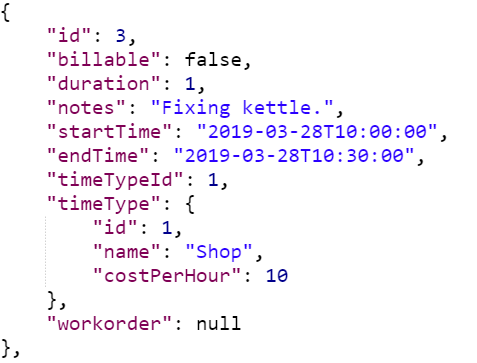
\includegraphics[width=4in]{JSON-post-recieve.png}\\
	\caption{A time entry in the from of a JSON response from the server. For a GET all request, all objects in the database will show}
	\label{fig:tobias}
\end{figure}

\paragraph{GET single request}
This request is very similar to a GET all request from above, but instead of retrieving all entries, the request only receives a single object, based on the id of the specific object. Using figure 1 as an example, a request would be made with the specific identifier of the object, which is 3, and the server can send the response as long as the server is capable to. 

\newpage
\paragraph{POST request}
A post request spends a JSON object to the server such that it the object can be added to the database. The data is filled out according to the structure of the object, though not each field is required to be filled out. The following image showcases a JSON request being sent to the server. 
\begin{figure}[H]
	\centering
	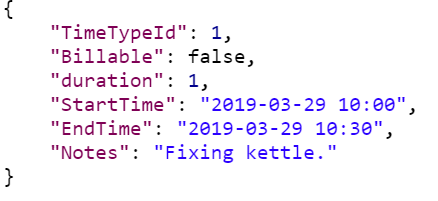
\includegraphics[width=4in]{JSON-post-send.png}\\
	\caption{A time entry JSON request to be sent to the server.}
	\label{fig:tobias}
\end{figure}

When a POST request was successful in being added to the database, a status code of 201 Created will be sent back and the object created will showcase much like a get request. Notice that the POST request did not have each field included. Certain fields that have embedded fields do not need to be specified, but rather referenced as they are already pre-populated at the time of the server being live. For example using figure 2, the field TimeTypeId references the identifier in the TimeType table in the database and retrieves all of the data in that table which is aligned with that id. Since in the example TimeTypeId is 1, all of the fields in the TimeType table associated with that id will load onto the JSON object. How it is stored can be viewed using figure 1 shown earlier. 

\paragraph{PUT request}
When a current entry in the database needs to be altered or edited in any capacity, a PUT request is sent to the system. This requests consists of a JSON object filled with the data that is to be changed and the id of the particular object in the database that will be changed. The request is sent to the specific id of the object, so that the changes are made to that specific entry. A successful return will send back a 204 No Content response, meaning that there was a successful response, but there the chandged data is not shown by the request. To view the changes, a GET request is required. 

\paragraph{DELETE request}
To delete an entry from the database, a DELETE request is sent to the system specifically by the id of the object to be deleted. On a successful response, the database will respond with a 200 OK and the JSON object, signalling that the object was successfully deleted and removed from the database. 

\subsubsection{Integration Testing}
Once each separate endpoint is tested by sending CRUD requests, the next set of tests look to see if the JSON object that require the use other objects that are created on run time are integrated correctly. For example, a time entry has a field regarding workorders and whether or not any are associated with the particular entry. When there are associated workorders, a POST request should be able to include the workoder id and be able to reference said workorder by said id. When a GET request is sent to view the time entry, the workorder that is referenced should appear as well. Integrated object such as these are to be tested such that each table can properly store and showcase these integrations. 

\subsubsection{Performance Testing}
After the competition of testing how each endpoint is integrated, further tests to indicate how quickly a request can be processed are done. While this type of tests are more thoroughly done after the competition of both frontend and backend testing, these tests backend exclusive performance tests are done to ensure that there exists a steady connection to the database and that requests a before being processed quickly without extended periods of latency before the requests are even processed by the frontend. 
\newpage

\subsection{Frontend Testing}
For the frontend section of the project, testing in general consists of visually inspecting whether or not certain elements of the frontend are being processed correctly as well as whether or not each page is formatted correctly. A large concern of the frontend is how the data will appear on the page once it is loaded from the backend. For Vue based project, Jest is a tool that allows the developer to create asserts to ensure that the data the frontend is expecting is in the proper format. This is done so that a particular page will expect and only allow specific data. 

\subsubsection{Unit Testing}
To test the appearance and styling of a particular page, the frontend is run on a development server provided by the Node Package Manager, or npm for short. This development server allows each page in the frontend to be loaded as a locally hosted webpage accessible by a web browser. While programming, the server will automatically update the current page being worked on, showcasing which changes are being made in realtime. By having an environment that can show results instantaneously, a particular page can be evaluated on the spot without having to switch from development mode to testing mode. Each error or bug can be fixed much more quickly. Whenever a page cannot be properly generated due to a particular bug or issue, the error is showcased on the page itself. As such, most of the testing is done to ensure that the page is loaded correctly in the way it was intended. 

\subsubsection{Integrated Testing}
These tests are similar to the unit tests in that all testing can be done simultaneously with development to ensure that each page in the frontend can direct and redirect the user to the proper destination page and that the navigation is smooth, logical and feasible.  

\subsubsection{Automated UI Testing}
These tests are currently not in the inital development schema but are to be implemented for future testing to ensure that the frontend can be automated smoothly and efficiently. Each test ensures that each page is possible to navigate to and each page loads all necessary information upon runtime.


\subsection{Integrated Testing}
Once both frontend and backend sections are tested fully, the front end and backend sections are integrated to gether such that the frontend can send requests to the backend and the backend can respond back. Essentially, the frontend has to be able to replace the functionality of Postman. 

\subsubsection{Unit Testing}
Similar to the frontend unit tests, these tests can be done during development, to ensure that the particular page has a stable connection to the database, is able to get a response when requesting objects from the database, and is able to properly  display that data where needed. The development server will showcase the result by loading the particular page and if developed correctly, the data received will display as intended. For example, when a time entry requested is properly received from the database, the data is mapped such that the entry can appear on a calendar in the page where it was requested. Each time a new entry is made, then the page will load that entry in the calendar if successful. 

\subsubsection{Performance Testing}
One the integration tests are all complete, the system will then undergo vigorous performance testing to ensure that each section of the site is able to load its data from the server as efficiently and as quickly as possible. Each page must be able to work as quickly as can be so that the user does not have to experience any latency during production. Each task and feature should be optimized by this effort. Once these tests are complete, the program is ready for release, but performance tests are never truly finished, as the program should run efficiently at all times and any bugs found during use can be patched quickly. 

\newpage
\section{Test Schedule}
As stated in the previous sections, the plan to test each endpoint of the backend first separately, progressing into endpoint integration testing. After such, frontend page unit and integration testing is to be done before full backend and frontend integration testing is completed. Once each section of testing is completed, the program is intended to undergo stress testing and production testing, with the application being constantly improved and worked on as bugs are found.

\subsection{Features to be Tested}
\subsubsection{Backend}
The most important aspects of the program will be undergoing testing as part of the first release. For the backend, it is essential that every endpoint is fully fleshed out and optimized, and as such each endpoint has an associated unit test. Each endpoint must be able to be accessed and data can be requested or sent over.   
\newline
{\setlength{\parindent}{0cm}

Endpoints with inherited data is also a feature that will be tested, such that each can reference and load the correct data from the database when requested. This is done so that when features that require data from multiple sources, such as workorders and the materials that will be used, and any time tracking information that it may come with. 

\subsubsection{Frontend}
On the frontend, the most important features are the ability to create and view workorders, create and view materials and create and view time entries. Each page should have its full ability to create and edit entries, and have each page related to the feature properly implemented at run time. As such, these main pages are the top priority of testing in the frontend section. 
\newline
{\setlength{\parindent}{0cm}
The side navigation bars which appear on each page of the frontend section also will be tested to ensure that each page can be accessed from these menus. This means that regardless of the page that the user is currently on, they are still able to navigate to any page of the application without having to backtrack. 

\subsection{Features not to be Tested}
The features that are in currently in development but will not see full implementation in the first release will not be tested. These main features are frontend features such as the report generation due to the implementation of these features not being able to be fully implemented and operational during the first release of the application. In the next release, once these features are implemented to their full potential, they will be added to the testing plan. Other features that will not be tested include retrieving pre populated data from the database. Since this data is constant and is only used by the system when it is referenced by an editable endpoint, the test to see if the data exist already is tested during the endpoint unit tests. 
\newline
{\setlength{\parindent}{0cm}

Testing the compatibility of the site to work on a mobile device will also not be currently tested as the application is originally designed to have to function primarily on a desktop or laptop. Since the application is run using a full scale web browser, the application was not originally intended to be used on a mobile device.

\section{Dependencies}
The system requires the use of a full scale web browser that supports javascript functionality and will not function on Internet Explorer 8 or below. This is due to the software requirements of ASP.NET and Vue.Js, the frameworks that the application was designed with. However, the application will be able to run on any type of personal computer operating system, as it is only limited by the type of browser the machine is using. The system does require a steady internet connection, as the frontend is constantly communicating with the backend, which will be hosted on a server that the application must have a steady connection to. 

\section{Risks and Assumptions}
The main assumption that is made while using this system is that the client is completely authorized to access all of the workorders and associated data to the engineering workshop. To reduce the risk of unauthorized use, the system does require a valid user login information before granting access. Another main assumption about the system is that all data that is currently entered to the system is relevant to the workshop in some capacity. It is the responsibility of the client to ensure that all data that is added by the client is done in a correct and proper manner.  

\section{Tools}
The main tool that used for testing is Postman, an API listening program that allows the testing environment to exists. The program acts as a requests hub, which will send requests directly to the backend and will await proper HTTP responses back, showcasing the result in a response window. It allows JSON objects to be sent to specific endpoints on the backend that will then populate the database during development. This allows for bakcend only development without the need of the frontend pages to be fully developed, allowing the refinement and proper implementation of each endpoint. The following figure showcases the program and how a request is made. 
\begin{figure}[H]
	\centering
	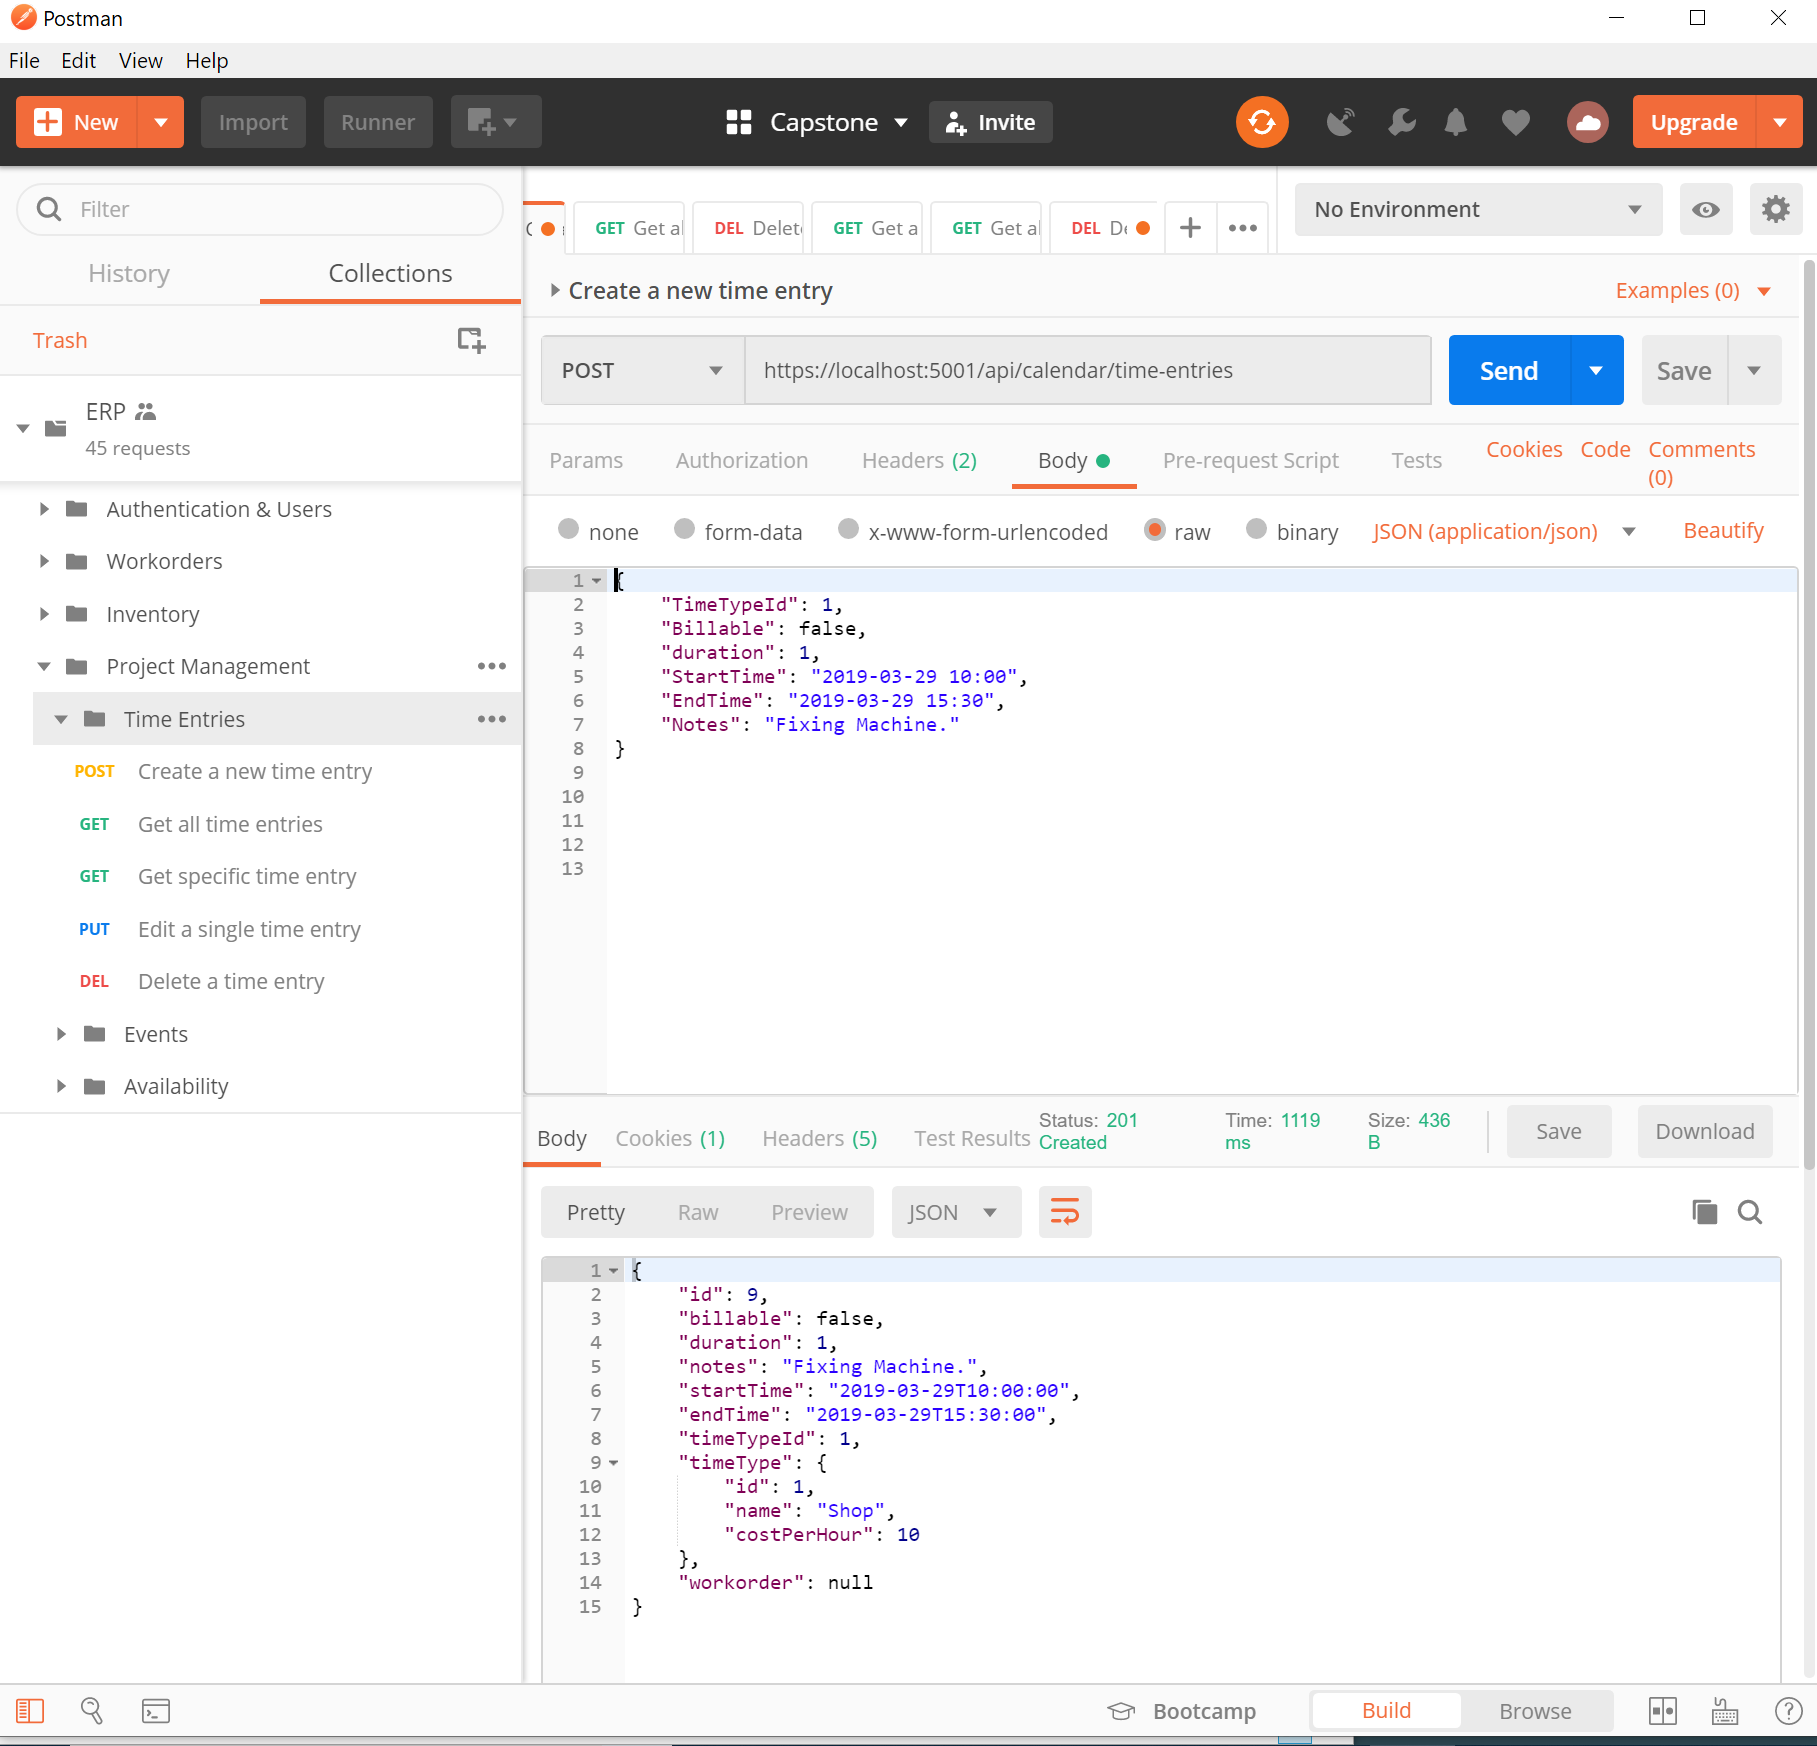
\includegraphics[width=5in]{Postman.png}\\
	\caption{Sending a POST request in Postman}
	\label{fig:tobias}
\end{figure}


On the frontend side, the main testing tool is the one used alongside development which is the Vue command line interface run serve, which allows the frontend to be run on a development server. This server allows for any changes during development of the frontend to appear instantaneously rather than having to reload the page after every change. This allows for quicker error checking and page evaluation, which in turn means that unit tests for the frontend can be done immediately after a feature is implemented.  In total, the frontend does not require many tools for testing, however the use of this development server does allow for more tests to be completed more quickly. The following figure showcases the development server running. Notice the URL of where the frontend is being run. 
\begin{figure}[H]
	\centering
	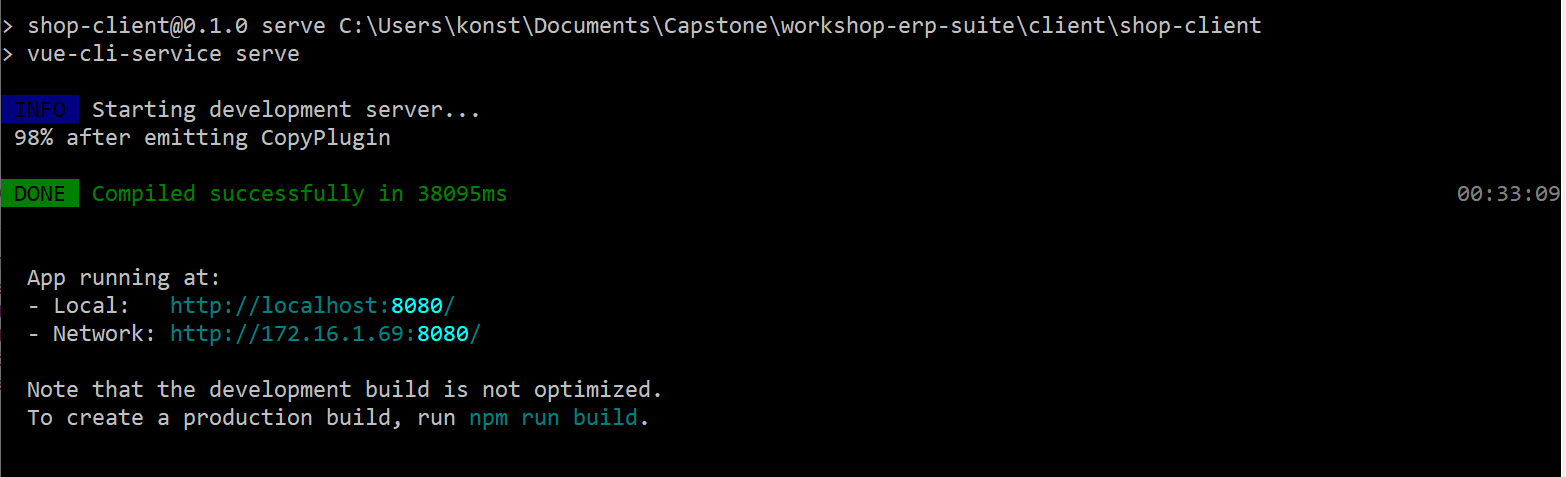
\includegraphics[width=4in]{Run-Serve.png}\\
	\caption{Development Server in use}
	\label{fig:tobias}
\end{figure}

\end{document}


